\documentclass[ngerman]{article}

\usepackage[margin=2.75cm]{geometry}
\usepackage[T1]{fontenc}
\usepackage[utf8]{inputenc}
\usepackage{textcomp}
\usepackage{graphicx}
\usepackage{babel}
\usepackage{titlesec}
\usepackage{xcolor}

%
% Paket fuer Links innerhalb des PDF Dokuments
%
\definecolor{LinkColor}{rgb}{0,0,0}
\usepackage[plainpages=false,hyperfootnotes=false]{hyperref}
\hypersetup{colorlinks=true,%
	linkcolor=LinkColor,%
	citecolor=LinkColor,%
	filecolor=LinkColor,%
	menucolor=LinkColor,%
	urlcolor=LinkColor
}


\title{Förderverein für Freie Netze in Hessen\\
-- Ziele und Vision --}

\begin{document}
\parindent 0pt
\parskip 10pt

\maketitle

Die Informationsgesellschaft unserer Tage ist ohne Computer und Datennetze nicht mehr denkbar.
In\-for\-ma\-tions- und Kommunikationstechnologien spielen eine wichtige Rolle für den Zugang zu Bildung, Kultur und Wissenschaft.
Trotz immer neuer und schnellerer digitaler Kommunikationsformen ist der Zugang zu diesen Technologien nicht allen Menschen gleichermaßen möglich.
Der Verein zur Förderung freier Netze Hessen hat sich zur Aufgabe gemacht, den Betrieb freier Funknetze zu fördern und dadurch den gleichberechtigten und nicht diskriminierenden Zugang zu Informationen, unabhängig von kommerziellen Interessen zu ermöglichen.
Dies wird erreicht durch den Aufbau und Betrieb einer entsprechenden Infrastruktur, sowie die Aufklärung der breiten Masse im Bezug auf die Auswirkungen freie zugänglicher Netze auf die Gesellschaft erreicht.


\section*{Was sind freie Funknetze}

In einem freien Funk-Netzwerk stellen alle Nutzerinnen und Nutzer ihre eigenen WLAN-Router für den Datentransfer der anderen Teilnehmer zur Verfügung.
Im Gegenzug können die Nutzerinnen oder Nutzer Informationen über das Netz übertragen oder von Teilnehmern eingerichtete Dienste im Netz nutzen.
Die Benutzer stellen somit auch gleichzeitig die Betreiber der Computernetzwerke dar, die von einfachen Heimnetzwerken ausgehend Häuser, Stadtteile, Dörfer oder ganze Städte vernetzen.
Durch das zur Verfügung stellen der Internetverbindung einiger Teilnehmer des Netzes, ermöglichen diese anderen Teilnehmern den Zugang zum Internet und somit zu Angeboten wie Wikipedia, Nachrichten-Portalen oder Online-Zeitschriften.

Mit der Realisierung freier Funknetze und der Weitergabe von Wissen zu diesem Thema beschäftigen sich der \textit{Förderverein freie Netzwerke e.V.} \cite{foerderverein}, sowie eine Vielzahl regionaler Verbände.
Die Arbeit dieser Verbände und Arbeitsgruppen, die einerseits die rechtlichen Rahmenbedingungen und andererseits die Entwicklung von Hard- und Software betreffen, wird unter dem Namen \textit{Freifunk} \cite{freifunk} zusammengefasst.
Alle Ergebnisse dieser Arbeit werden der Öffentlichkeit unter freien Lizenzen zur Verfügung gestellt, um sowohl die Verwendung als auch die Beteiligung an der Weiterentwicklung zu ermöglichen. 

\section*{Wie lassen sich solche Netze realisieren} 

Zur Realisierung verwenden die \textit{Freifunk-Projekte} Standard-WLAN-Router (Knoten), die aus dem privaten Hausgebrauch bekannt sind.
Diese werden mit einer speziellen Freifunk-Firmware (das Betriebssystem des WLAN-Routers) ausgestattet, die dezentral in den regionalen Freifunk Verbänden entwickelt wird.
Änderungen und Erweiterungen, die in einem regionalen Verband durchgeführt werden, stehen anschließend wiederum allen Verbänden zur freien Nutzung und Modifikation zur Verfügung.

Ein mit der Freifunk-Firmware ausgestatteter WLAN-Router ist in der Lage, weitere Freifunk-Knoten in seiner Nähe automatisch zu erkennen und sich mit diesen per WLAN zu verbinden.
Es entsteht ein sogenanntes WLAN-Mesh-Netzwerk \cite{wlan-mesh}, das sich dadurch auszeichnet, dass jeder Knoten mit einer Vielzahl anderer Knoten verbunden ist.
Mit Hilfe eines intelligenten Routing-Protokolls, das speziell für unzuverlässige Funknetze entworfen wurde und ebenfalls unter einer freien Lizenz zur Verfügung steht, ist die Wegfindung innerhalb des Netzes und somit die Kommunikation untereinander möglich.
Durch die Verbindung jedes Knoten mit einer Vielzahl gleichberechtigter Knoten entsteht ein sehr robustes regionales Datennetz.

\begin{figure}[h]
	\centering
	\fbox{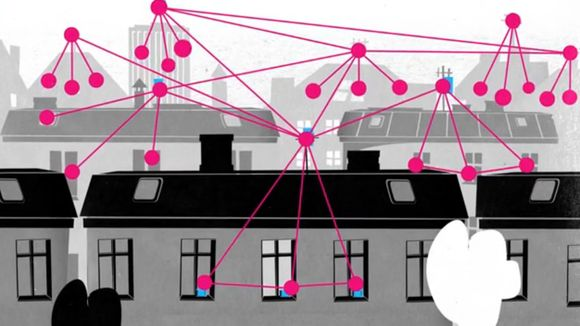
\includegraphics[width=.8\textwidth]{freifunk-mesh}}
	\caption{Schematische Darstellung eines regionalen WLAN-Mesh-Netzes}
	\label{fig:freifunkwolke}
\end{figure}

Abbildung \ref{fig:freifunkwolke} zeigt, wie durch den Betrieb von Freifunk-Knoten in den Wohnungen von Bürgern ein miteinander verbundenes Netzwerk entsteht, das unabhängig von kommerziellen Anbietern funktioniert.
Nutzer, die sich mit dem Freifunk-Netz verbinden, können untereinander kommunizieren und Daten austauschen, ohne dass dazu ein Internetanschluss benötigt wird.



\section*{Wie wird das vom Förderverein Freie Netze Hessen umgesetzt}

Der Förderverein für Freie Netze in Hessen bietet eine Plattform um Interessierten das Wissen für den Aufbau und Betrieb von freien Netzen zu vermitteln und dadurch Freifunk in Hessen aktiv zu unterstützen.
Er erreicht dies durch die Zusammenführung von Menschen, denen er den Informationsaustausch untereinander gestattet und damit gegenseitige Hilfestellung beim Erlernen der technischen Grundlagen und dem Aufbau von Infrastruktur freier Funknetze ermöglicht. 
Darüber hinaus richtet sich der Verein durch Publikationen und die Durchführung von Vorträgen und Workshops direkt an die Bürger in Hessen, um diese über mögliche Vor- und Nachteile freier Funknetze aufzuklären.

Zu den konkreten Themen zählen unter anderem die folgenden Aspekte:
\begin{itemize}
	\item Sicherer Betrieb von Netzwerkinfrastruktur und Diensten (u.a. auch im Internet),
	\item Sicherheit und Datenschutz bei der Nutzung öffentlicher Datennetze (u.a. auch im Internet)
	\item Effizienter und Ressourcenschonender Betrieb von Funk-Netzwerken
	\item Vermittlung wissenschaftlicher Erkenntnisse zu gesundheitliche Risiken
	\item Förderung gemeinschaftlichen, interdisziplinären Arbeitens bei Planung, Aufbau und Betrieb der Infrastruktur
	\item Vermittlung von Wissen zur Verwendung freier Software
	\item Hilfestellung bei der Beteiligung an der Entwicklung freier Software
\end{itemize}

\color{red}
ToDo:\\
- Abschließenden Satz finden / irgendwie abrunden\\
- aus der Aufzaehlung ggf. Fliesstext machen\\
- weitere Aspekte?

\color{black}
\begin{thebibliography}{1}
	\bibitem{foerderverein} Förderverein freie Netzwerke e.V. -- \url{http://foerderverein.freie-netzwerke.de}
	\bibitem{freifunk} Wikipedia zu Freifunk -- \url{http://de.wikipedia.org/wiki/Freifunk}
	\bibitem{wlan-mesh} Wikipedia zu Ad-Hoc-Netz -- \url{http://de.wikipedia.org/wiki/Ad-hoc-Netz}
\end{thebibliography}


\end{document}